\documentclass[12pt]{article}

\usepackage{times}
\usepackage{amssymb,amsmath}
\usepackage{graphicx}
\usepackage{subfigure}
%\usepackage{verbatim}
\usepackage{hyperref}
%\usepackage{doublespace}
%\usepackage{lineno}

%-------------- editing ----------------------
\usepackage{color}
\newcommand{\comment}[1]{\textcolor{blue}{[ \sc{#1} ]}} % comments
\newcommand{\revise}[1]{\textcolor{black}{{#1}}} % revisions
%\usepackage{ulem}
%---------------------------------------------

\begin{document}
%\linenumbers

\title{
Vehicular Mobility in San Francisco
}

\author{Jonathan W. Lee}

\date{\today}

\maketitle

\section{Motivation}
As urbanization, vehicular dependence, and fuel consumption continue to grow into the future, mobility within cities becomes an increasingly relevant dilemma. Large metropolitan areas like Los Angeles, New York City, and Washington, D.C. are notorious for terrible traffic conditions. Los Angeles conditions are particularly problematic as many carpool lanes are in effect 24/7, as opposed to the typical rush hour period in most cities. Traffic has direct impacts on commute times, road safety, energy consumption and dependence, etc., not to mention countless intangible impacts. This project is aimed at evaluating the traffic problem from a mobility perspective.

\section{Introduction}

In my preliminary search, I have found two data sets which will serve as the basis for my project. The first contains archived anonymized GPS traces from Uber -- 
time of day, day of week, latitude, and longitude of 25,000 trips in San Francisco, logged every four seconds. The data has been anonymized by truncating the 
beginning and end of every trip and removing the actual dates of the trips. The second data set contains GPS traces of SF MTA buses -- date, time, latitude, 
longitude, heading, and speed, logged every 90 seconds over the last three months.

\begin{figure}[hbtp]
\caption{\label{fig:overlay}An overlay of Uber (orange) and SF MTA (red) GPS traces in San Francisco.}
\begin{center}
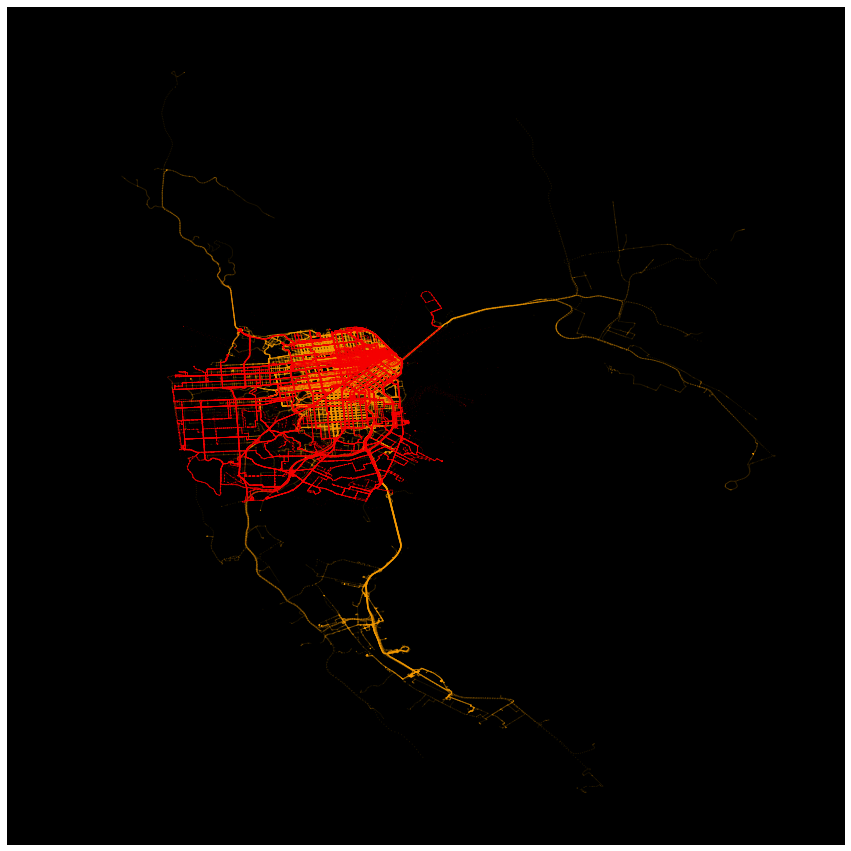
\includegraphics[width=5in]{overlay.png}
\end{center}
\end{figure}

In addition to the above data sets, I may also include sources from topography data and/or SF traffic shape files. It would also be nice to include influences from 
weather, but correlation with the Uber data may be difficult since the Uber data has been anonymized (\textit{i.e.}, dates are modified).

From these data sets, my goal is to obtain a better understanding of the traffic flow in San Francisco. I plan to characterize traffic in the city of San 
Francisco as a function of day of week, time of day, and location. Further, I would like to categorize anonymous Uber drivers by driving behavior. Finally, I 
would like to develop a model to predict fuel consumption. To achieve these goals, I will need to derive several intermediary variables from those provided in 
the data sets:

\begin{itemize}
\item traffic: create new metric from bus data
\item Uber velocity: time derivative of Uber position, interpolated and extrapolated from half time steps to full time steps
\item Uber acceleration: second time derivative of Uber position
\item Uber mean free path: average path length from acceleration to deceleration
\item Uber uniformity of speed: decay rate of velocity autocorrelation
\end{itemize}


\section{Data Project}

With the above variables established, I propose three projects, each compounding upon the previous.

\begin{enumerate}

\item \textbf{Project 1}: I will first create a model for fuel consumption, which will be approximately proportional to an integral of positive accelerations. 
Alternatively, for electrified vehicles, electricity consumption may also be computed by subtracting some integral of negative accelerations to model 
regenerative braking. It may also be influenced by topography (\textit{e.g.}, accelerating uphill, regenerating downhill, etc.). Secondly, I will use 
\textit{k}-means clustering to categorize Uber driver behavior. Clustering will be based on all the engineered features listed above. This will allow me to find 
the relationship between categorized driving behaviors and fuel economy.

\item \textbf{Project 2}: I will build a routing algorithm, given starting location, destination, day of week, time of day, and driving behavior. The base 
algorithm will use Dijkstra's algorithm, however it will be modified to present multiple route options, \textit{e.g.}, fastest route, most direct, best fuel 
economy, least congestion, etc.

\item \textbf{Project 3}: I will build a mobility map of San Francisco. The tool will take as inputs starting location, day of week, time of day, travel time, 
and driving behavior (based on the clustering in Project 1). As output, it will present a highlighted area of all potential destinations that are reachable in 
the given travel time. Versions of this have already been implemented, \textit{i.e.}, Isoscope and Trulia. However, Isoscope is limited to 10 minute trips, 
Trulia has no time dependence feature (presumably limited to commute hours), and neither factor in driving behavior. Additionally, my tool will report (via 
color) the fuel/electricity consumed for all destinations at the boundary. To find the potential destinations, I will use some modified form of Dijkstra's 
algorithm. Cumulative travel time and consumed fuel will be tracked as the algorithm proceeds.

\end{enumerate}

\end{document}
